
\chapter{راهکار پیشنهادی}

در این فصل یک راهکار پیشنهادی ارائه کرده و نتایج آزمایش های کوتاه مدت روی این معماری پیشنهادی را مطرح می‌کنیم.

\section{تعریف مدل پیشنهادی}

تصویر ورودی را به صورت $I \in \mathbb{R}^{H \times W \times C}$ در نظر بگیرید که $H$ و $W$ به ترتیب ارتفاع و عرض تصویر و $C$ تعداد کانال‌ها (مانند ۳ در تصاویر \lr{RGB}) است. همچنین هدف ترمیم (ماسک) را با
$M \in \{0,1\}^{H \times W \times 1} $
نشان می دهیم به طوری که ۰ نواحی از دست رفته (هدف ترمیم) و ۱ نواحی موجود را نشان می‌دهد. همچنین برای سادگی محاسبات و توضیحات فرض کنید $H$ و‌ $W$ هر دو برابر و بر $P$ بخش‌پذیر هستند (تصویر ورودی مربعی است). برای پردازش تصویر، ابتدا آن را به $N$ قطعه (پچ) با ابعاد $P \times P$ تقسیم می‌کنیم، به‌طوری‌که تعداد کل پچ‌ها از رابطه زیر به دست می‌آید:
$$
N = \frac{HW}{P^2}
$$

$N$
قطعه به دست خواهند آمد که هر قطعه شکلی در ابعاد ${P \times P \times C}$ خواهد داشت.
$$
I\_{patches} \in \mathbb{R}^{N \times P^2 \times C}
$$

با مسطح کردن هر قطعه، یک بردار 
$x_i \in \mathbb{R}^{P \cdot P \cdot C}$
برای هر قطعه $i$ داریم. یعنی تصویر ورودی به دنباله ورودی زیر تبدیل می‌شود:
\[
X_P = [x_1, x_2, \dots, x_N] \in \mathbb{R}^{N \times (P^2 \cdot C)}
\]

\begin{figure}
	\centering
	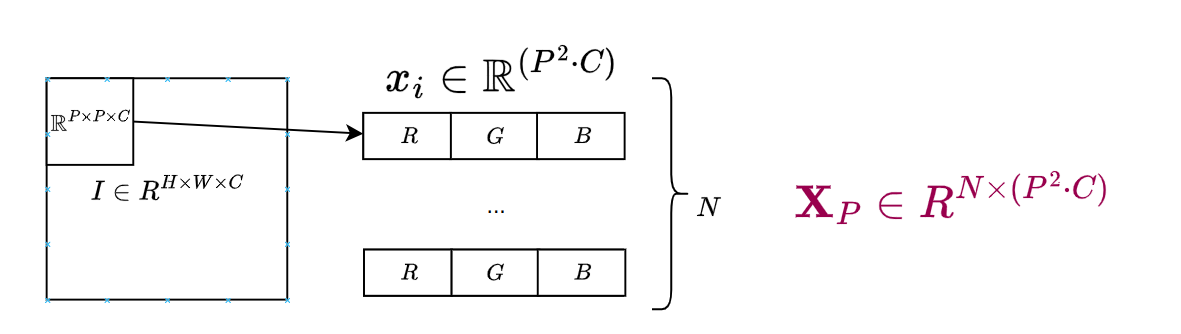
\includegraphics[width=0.7\linewidth]{decompose}
	\caption{نحوه تجزیه تصویر و تبدیل آن به یک دنباله برای ورود به ترنسفورمر (بعد از اعمال یک نگاشت خطی)}
	\label{fig:decompose}
\end{figure}

به‌منظور تبدیل این دنباله به فضای نهان ترنسفورمر، نگاشت خطی قابل‌آموزش زیر را تعریف می‌کنیم
\begin{equation}
	E\_{enc} \in \mathbb{R}^{(P^2 \cdot C) \times D\_{model}}
\end{equation}

که در آن $D\_{model}$ بعد فضای نهان مدل است. پس از آن مانند قبل جاسازی‌های موقعیتی را اضافه می‌کنیم (روش پیشنهادی ما از جاسازی های سینوسی ثابت استفاده میکند، نه جاسازی های قابل یادگیری).
%\footnote{نمونه ای از اعداد مناسب برای این بعد ۱۲۸، ۵۱۲ یا ۱۰۲۴ است. بدیهی است ابعاد بیشتر ویژگی های بیشتری یاد گرفته ولی هزینه پردازش را به‌شدت افزایش می‌دهند.}
نتیجه نگاشت خطی به صورت زیر خواهد بود:
$$
X = X_P \cdot E\_{enc} + PE \in \mathbb{R}^{N \times D\_{model}}
$$

\subsection{ماتریس ماسک توجه}


برای همگام‌سازی ماسک ورودی با پچ‌های تصویر، ماسک اصلی 
$ M \in \{0,1\}^{H \times W \times 1} $
به
$ M' \in \{0,1\}^{N} $
تبدیل می‌شود. در این تبدیل، اگر حتی یک پیکسل در هر پچ (با ابعاد \( P \times P \)) ماسک شده باشد، کل پچ در \( M' \) ماسک‌شده (دیده نشده) و برابر با ۰ در نظر گرفته می‌شود.
% CHECK ESPECIALLY THE DIMENSIONS. I COULD HAVE MESSED UP REAL BAD.
$$
M'_i = \min \{ M[x, y] \mid (x, y) \in \text{\lr{patch }} i \} \in {\{0,1\}}^{N}
$$
که در آن $ m'_i $ عنصر $i$-ام از بردار  $M'$ است و متناظر با $i$-امین قطعه $ x_i$  می‌باشد.

یک راه خلاقانه پیاده‌سازی این تبدیل استفاده از عملیات MinPooling با اندازه هسته $P$ و گام $P$ است. (شکل \ref{fig:maskconv1})
$$
M' = \text{Flatten}(\text{MinPool}(M, P, P)) \in {\{0,1\}}^{N}
$$


سپس $M'$ به یک ماتریس دو بعدی مثل $ A = a_{ij} $ تبدیل می‌شود تا برای هر جفت پچ مشخص کنیم که آیا آن‌ها می‌توانند به یکدیگر توجه کنند یا خیر. در این ماتریس دو بعدی که به آن ماسک توجه
\LTRfootnote{Attention Mask}
گفته می‌شود، اگر هر دو قطعه \( i \) و \( j \) قابل مشاهده باشند (یعنی \( m'_i = m'_j = 1 \))، پس آن‌ها می‌توانند به یکدیگر توجه کنند. در این صورت، در ماتریس توجه، مقدار آن‌ها برابر با مقدار عادی خواهد بود. همچنین یک قطعه ماسک شده «باید» به قطعات ماسک نشده توجه کند. این بنیه اساسی ترمیم کننده بر پایه ترنسفورمر است. اما بسیار مهم است که قطعه های سالم به قطعه های ماسک شده توجه نکنند. چون اطلاعاتی دریافت نمی‌کنند و در این صورت باید توجه بین آن‌ها مسدود شود. به عبارت دیگر، مقدار آن‌ها باید به منفی بی‌نهایت تغییر کند تا مدل از توجه قطعات سالم به قطعات ماسک شده بپرهیزد.

فرم ماتریس ماسک توجه مانند $ A = a_{ij} $ بدین صورت است که $a_{ij}$ مشخص میکند آیا موقعیت $i$ (پرسش) حق دارد به موقعیت $j$ (کلیدها) توجه کند یا خیر؟ اگر مجاز بود، آن درایه ماتریس عدد 0 (بدون پنالتی) و اگر مجاز نبود $- \infty$ (پنالتی بینهایت) در آن درایه می‌نشیند. سپس پس از محاسبات امتیاز های توجه،‌ A به آنها اضافه می‌شود.
با توجه به موضوع مطرح شده، ماتریس توجه برای عملیات ترمیم بدین صورت تشکیل می‌شود:

% full-patch observation masking (all pixels in a patch must be observed to use it).
$$
A_{i,j} = \begin{cases} 
	0 & \text{\lr{if }} M'_j = 1 \quad (\text{\lr{key }} j \text{\lr{ is visible}}), \\
	-\infty & \text{\lr{if }} M'_j = 0 \quad (\text{\lr{key }} j \text{\lr{ is masked}}).
\end{cases}
$$

%
%For healthy queries (i=1), they can attend to healthy keys (j=1) — correct.
%
%- For masked queries (i=0), they can attend to healthy keys (j=1) — correct, as they need to gather information.
%
%- All queries (i=1 or i=0) cannot attend to masked keys (j=0) — correct, since masked keys have no information.

\begin{figure}
	\centering
	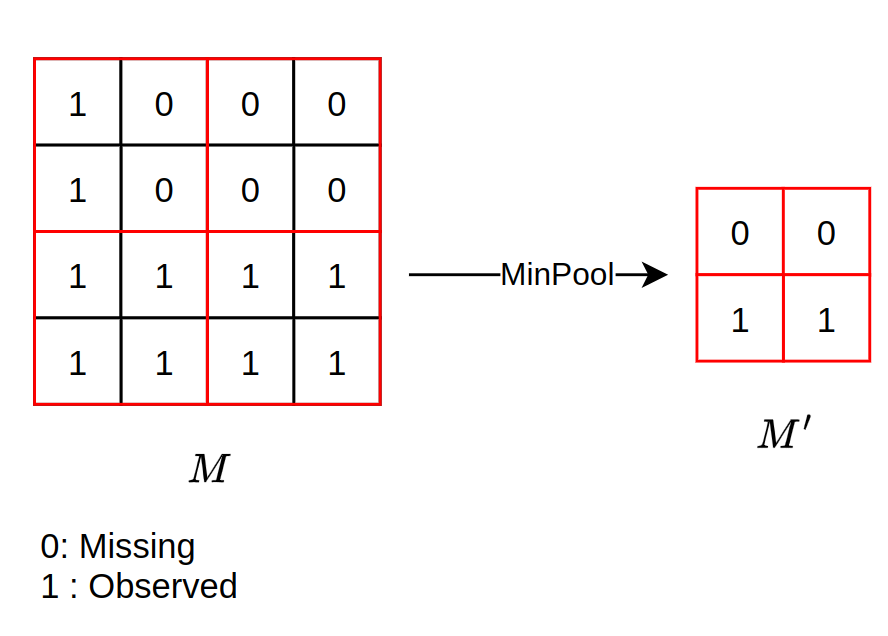
\includegraphics[width=1\linewidth]{maskConv1}
	\caption{تبدیل ابعاد ماسک با روش پولینگ}
	\label{fig:maskconv1}
\end{figure}

\subsection{بلوک توجه}
%به منظور راحتی در محاسبات با اعداد تعریف‌شده، هم اکنون با توجه به خاصیت های این مجموعه‌داده برخی پارامتر های معماری را تثبیت می‌کنیم:
به تعداد $h$ «سر» توجه می‌سازیم. معمولا رابطه زیر بین تعداد سر ها و ابعاد نهان هر سر برقرار است. اما مدل ما منطف است و الزامی برای چنین رابطه ای ندارد.
\begin{align*}
	D\_{head} = D\_{model} / h
\end{align*}

امتیاز هر سر بصورت زیر محاسبه خواهد شد:

\begin{align*}
	\mathbf{Q}_i &= \mathbf{X} \mathbf{W}_i^Q \in \mathbb{R}^{N \times D\_{head}}, \\
	\mathbf{K}_i &= \mathbf{X} \mathbf{W}_i^K \in \mathbb{R}^{N \times D\_{head}}, \\
	\mathbf{V}_i &= \mathbf{X} \mathbf{W}_i^V \in \mathbb{R}^{N \times D\_{head}}.
\end{align*}
در اینجا از پیاده‌سازی توجه نقطه‌ای مقیاس‌شده استفاده کردیم  و ماسک $A$ را اینجا استفاده می‌کنیم تا روابط غیرمجاز (مثلا توجه بخش‌های سالم به بخش‌های نیازمند ترمیم) را پنالتی کنیم. هر «سر» امتیاز توجه خود را در یک زیرفضا محاسبه می‌کند و در نهایت به همدیگر الحاق می‌شوند. نتیجه الحاق توسط نگاشت خطی 
$\mathbf{W}^O\in  \mathbb{R}^{h \cdot D\_{head} \times D\_{model}}$ 
به ابعاد خروجی استاندارد منتقل می‌شود. (با توجه به تقسیم 
$D\_{model}$ ضرب $h \cdot D\_{head}$
همان $D\_{model}$ است. اما تقسیمات دیگری هم برای «سر» های توجه ممکن هستند.)
\begin{align}
	\text{head}_{i} =
	\text{Softmax}\left(\frac{\mathbf{Q} \mathbf{K}^\top}{\sqrt{D\_{head}}} + \mathbf{A} \right) \mathbf{V} \in \mathbb{R}^{N \times D\_{head}}
\end{align}
\begin{gather*}
	\text{Concat}(\text{head}_1, \text{head}_2, \dots, \text{head}_H)  \in \mathbb{R}^{N \times (h \cdot D\_{head})} \\
	\text{MultiHead}(\mathbf{X}) = \text{Concat}(\text{head}_1, \dots, \text{head}_h)\mathbf{W}^O  \in \mathbb{R}^{N \times D\_{model}}
\end{gather*}

پس از اعمال توجه چندگانه به ورودی $X$، نتیجه‌ی آن با ورودی اولیه $X$ از طریق یک اتصال چسبنده ترکیب می‌شود و سپس خروجی نرمال‌سازی لایه‌ای می‌شود. هدف بهبود جریان گرادیان هاست. 
$$
X_{\text{\lr{norm1}}} = \text{LayerNorm}(X + \text{MultiHead}(X)) \in \mathbb{R}^{N \times D\_{model}}
$$

در قدم بعدی یک شبکه کاملا متصل اضافه می‌کنیم که از فعال‌سازی GELU استفاده می‌کند. هدف استخراج ویژگی ها از خروجی ترنسفورمر است:
$$
\text{FFN}(X_{\text{\lr{norm1}}}) = \text{GELU}(X_{\text{\lr{norm1}}} W_1 + b_1) W_2 + b_2 \in \mathbb{R}^{N \times D\_{model}}
$$
به‌طوری که دو ماتریس $W_1 $ و $W_2 $ قابل یادگیری هستند.
\begin{align*}
	W_1 \in \mathbb{R}^{D\_{model} \times D\_{fcn}},\\
	W_2 \in \mathbb{R}^{D\_{fcn} \times D\_{model}}.
\end{align*}
و در اینجا $D\_{fcn}$ بعد نهان لایه ی FFN است.  در هنگام پیاده‌سازی، یک لایه Dropout نیز اضافه می‌کنیم تا از بیش‌برازش جلوگیری شود. سپس در نهایت بار دیگر خروجی FFN را از یک لایه چسبنده +‌ نرم‌لایه ای می‌گذرانیم.
$$
X_{out} = \text{LayerNorm}(X_{\text{\lr{norm1}}} + \text{FFN}(X_{\text{\lr{norm1}}})) \in \mathbb{R}^{N \times D\_{model}}
$$

عملیات های ذکر شده (توجه چندگانه، سپس شبکه های پیش‌خور و چسبنده) را \textbf{بلوک توجه} می‌نامیم. هر بلوک توجه دارای ورودی با ابعاد $ N \times D\_{model} $ و خروجی با همین ابعاد است. یعنی هر بلوک توجه را می‌توان به دفعات تکرار کرد و پشت سر هم گذاشت.

\subsection{بازسازی نهایی تصویر}
نگاشت خطی قابل یادگیری $E\_{dec}$ را چنان تعریف می‌کنیم که 
$$
E\_{dec} \in \mathbb{R}^{D\_{model} \times P^2 \cdot C}
$$

با اعمال آن روی خروجی بلوک (های) توجه داریم
$$
\hat{X}\_{Flat} = X\_{out} \cdot E\_{dec} \in \mathbb{R}^{N \times (P^2 \cdot C)}
$$

با تغییر شکل (Reshape) هر قطعه به سه بعد با همان ابعاد ابتدایی و سپس بازسازی تصویری با ابعاد اولیه داریم:
$$
\hat{x}_i \in \mathbb{R}^{P^2 \cdot C} \quad \Rightarrow \quad \hat{x}_i \in \mathbb{R}^{P \times P \times C}
$$
$$
\hat{I} = \mathbf{Reshape}(\hat{X}\_{Flat}) \in R^{H \times W \times C}
$$
سپس از ماسک استفاده کرده و تنها بخش های ترمیم شده را به تصویر اصلی اضافه می‌کنیم.
$$
I\_{restored} = (\mathbf{M} \odot I\_{observed}) + ((1-\mathbf{M}) \odot \hat{I})
$$

\section{آموزش و پارامتر ها}

ما راهکار خود را روی یک برش ۵ هزار تصویری از مجموعه‌داده \lr{Danbooru2019 Portraits} 
\cite{danbooru2019Portraits}
شامل ۶۵ هزار تصویر دو بعدی کارتونی (به‌دلیل جزئیات ساده تر نسبت به تصاویر واقعی و امید به همگرایی سریع‌تر) آموزش دادیم که در آن  تصاویر $ 512 \times 512 $ هستند.  به دلیل نبود سخت افزار مطلوب و برای استخراج نتایج کوتاه‌مدت، آن ها را به $128 \times 128 $ ریسایز کردیم.

مدل پیشنهادی ما از ۴‌ «سر توجه» استفاده خواهد کرد و ابعاد نهان مدل ترنسفورمر را ۵۱۲ می‌گیریم ($D\_{model} = 512 $). ابعاد هر قطعه را 8 در 8 می‌گیریم ویعنی هر تصویر در ۱۰۲۴ قطعه بیان می‌شود ($N = 1024 $).
برای شبکه های کاملا متصل FCN، بعد نهان $D\_{fcn}$ را  2048 در نظر می‌گیریم (
$D\_{fcn}  = 4 D\_{model} = 2048$
)

\subsection{بهینه سازی}

می‌دانیم تابع هزینه \lr{L1} بدون ماسک بشرح زیر است:
$$
\mathcal{L}\_{L1} = \frac{1}{HWC} \| I\_{reconstruct} - I\_{gt} \|_1
$$
حال ما علاقمندیم تا اختلاف ها فقط در نواحی ای که مدل درحال بازسازی است محاسبه شوند.
\subsubsection{تابع هزینه \lr{L1} ماسک شده}

ماسک $\mathbf{M}$ مقدار ۱ را در نواحی معتبر و مقدار ۰ را در نواحی نامعتبر دارد. بنابراین، معکوس آن، یعنی $1 - \mathbf{M}$، فقط در نواحی‌ای که مدل باید بازسازی کند مقدار ۱ خواهد داشت. فرض کنید $\hat{I}$ تصویر بازسازی‌شده و $I$ تصویر حقیقت زمینه باشد. نرم یکم یک بردار جمع مقادیر مطلق تمام عناصر بردار است و نرم یکم یک ماتریس جمع مطلق درایه های آن است (
$\|Z\|_1​=\sum_i{|Z_i|}$
)  تابع هزینه‌ی پیشنهادی ما بصورت ترکیبی از اختلاف کل تصویر و ناحیه های ماسک شده، به‌صورت زیر تعریف می‌شود:

\begin{gather}
	\mathcal{L}_\text{mask} = \frac{ \| (1-M) \odot (I_\text{reconstruct} - I_\text{gt}) \|_1 }{ \| 1-M \|_1}, \\
	\mathcal{L}_\text{global} = \| I_\text{reconstruct} - I_\text{gt} \|_1, \\
	\mathcal{L}_\text{total} = \alpha\, \mathcal{L}_\text{mask} + \beta\, \mathcal{L}_\text{global}.
\end{gather}

در پیاده سازی خود، ما مقدار $\alpha$ و $\beta$ را ۱ در نظر گرفته ایم. اما  این مقادیر می‌توانند با انجام آزمون و خطا بهبود یابند تا تعادلی مناسب میان یادگیری ساختار کلی تصویر و توانایی ترمیم بدست آید.

مرتبه نرم برداری رابطه بالا یک است. اما می‌تواند برابر با ۲ برای پیاده سازی \lr{L2 loss} هم انتخاب شود. تفاوت ها و کاربرد های هر کدام در فصل دوم بیان شده است. ما از نرم اول استفاده کردیم. آزمایشات کوتاه مدت نشان دادند که با توجه به این که مدل در حال بازسازی کل قطعه های تصویر است،‌ استفاده از تابع هزینه ای که ماسک نشده باشد، تقلید کورکورانه را در مدل ترویج می‌دهد چون امتیاز «تشابه» از بخش های ماسک نشده بدست می آید و بازسازی نواحی ماسک شده ترویج نمی‌شود. پس لزوم دارد که تابع هزینه ماسک شود.

در عین حال، ما باور داریم برای این که مدل بتواند ماسک خوبی بسازد، ابتدا باید به اندازه‌ای تصویر را درک کرده باشد تا بتواند نواحی مشاهده شده - که در هنگام تست به آن داده می‌شود - را به خوبی بازسازی کند. این امر بدیهی ست زیرا اگر مدل نتواند قسمت های سالم را با کیفیت مطلوب پروکسی کند، یعنی ساختار تصاویر مجموعه‌داده ورودی را به خوبی یاد نگرفته است (که برای ترمیم با ماسک های بزرگ لازم است).

از آنجایی که روش ما مبتنی بر وصله های غیر همپوشان (
\lr{Non Overlapping}
) است، می‌توانیم از یک لایه UNet برای ترمیم لبه ها استفاده کنیم. یعنی  برای خروجی نهایی داریم:
\begin{equation}
	\hat{I} = CNN(X\_{out}) \in \mathbb{R}^{H \times W \times C}
\end{equation}

با استفاده از این روش، آزمایشات کوتاه‌مدت نتایج بهتری دادند اما نیازمند آموزش طولانی تری هستند و می‌توانند یک گلوگاه در کیفیت تصاویر خروجی باشند.

\section{جمع بندی}
در این فصل یک معماری ترمیم مبتنی بر ترنسفورمر را ارائه دادیم و توجیه کردیم و باور داریم که در صورت بهینه سازی هایپرپارامتر های مدل و فرایند یادگیری مناسب با سخت افزار مطلوب، این می‌تواند وابستگی های بلند مدت را بهتر از مدل های کلاسیک کانولوشنی استخراج کند.

یکی از نقاط ضعف مدل پیشنهادی، هدررفت اطلاعات در پچ هایی با چگالی ماسک کم است. در ساخت $M'$ اینطور عمل کردیم که اگر در هر قطعه حتی یک پیکسل در $M$ موجود بود، آن قطعه را به طور کل ماسک شده فرض کردیم. این فرض در ماسک های تُنُک خوب عمل نخواهد کرد چرا که بسیاری از قطعه ها با اطلاعات ارزشمند ماسک خواهند شد. اما این فرایند اجازه داد تا به تعادلی در هزینه های محاسباتی و جلوگیری از مشکلات ناشی از Downsampling برسیم.

اطلاعات بدست آمده می‌تواند پیش‌زمینه ای برای ظهور بیشتر مدل های ترمیم مبتنی بر ترنسفورمر  باشد. امیدواریم تا در تحقیقات آینده با بهبود مشکلات مدل فعلی، در بهبود این روش ها سهیم باشیم.

\textbf{پیاده سازی کامل این شبکه با استفاده از Tensorflow در کنار این فایل پیوست شده است.}


\begin{figure}
	\centering
	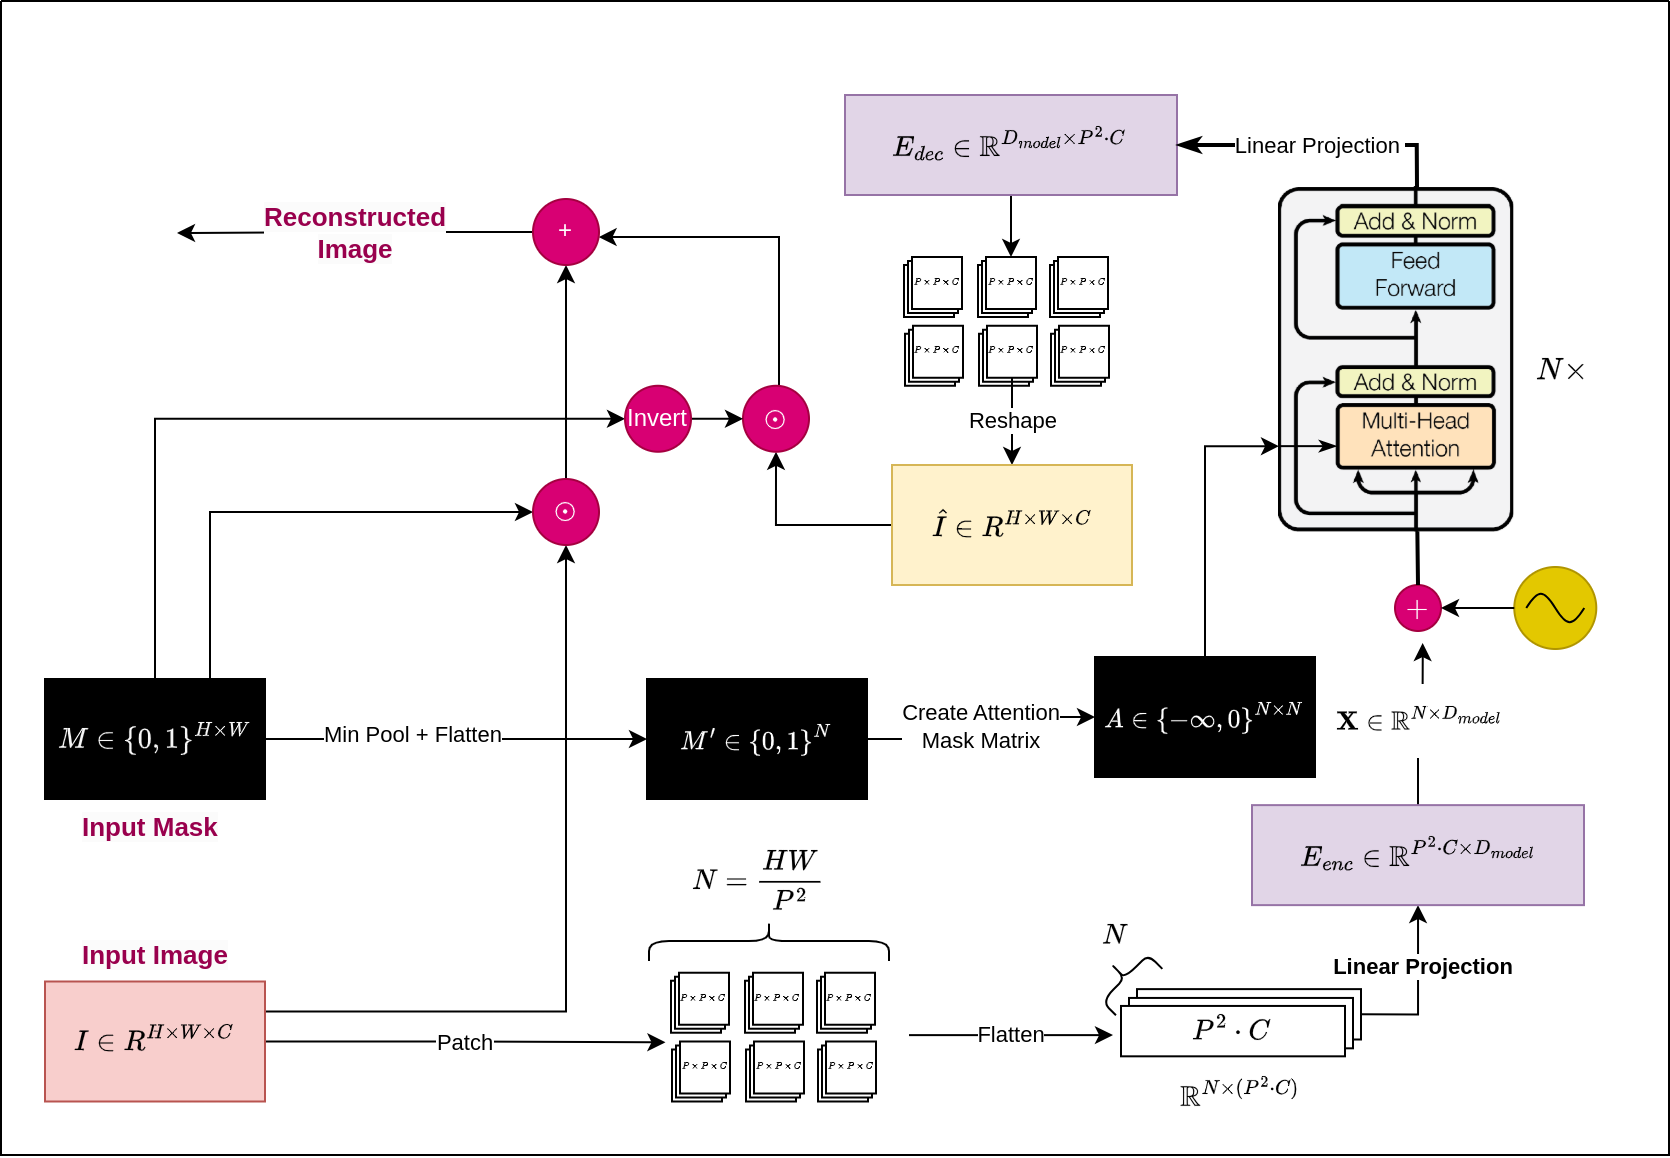
\includegraphics[width=1\linewidth]{ourarch1}
	\caption{معماری پیشنهادی ترمیم تصویر مبتنی بر وصله پیشنهادی ما}
	\label{fig:ourarch1}
\end{figure}